\chapter{Mise en \oe{}uvre et captures d'écran}
\label{chap:mise_en_oeuvre}

\section{Introduction}

Ce chapitre présente, à travers des captures d'écran, le fonctionnement réel de l'outil
NetSentry développé durant le stage, à partir d'un scan effectué sur un réseau local de
test : tableau de bord, détail d'un appareil, alertes, historique des scans, ainsi que
l'historique de versionnage du projet sur GitHub.

\section{Tableau de bord}

Le tableau de bord constitue le point d'entrée principal de l'application. Il présente
l'ensemble des appareils détectés sur le réseau, leur statut (en ligne / hors ligne), le
nombre total d'appareils ainsi que le nombre d'appareils non encore vérifiés
(\textit{unreviewed}), et permet de déclencher un scan manuel en un clic.

\begin{figure}[htbp]
    \centering
    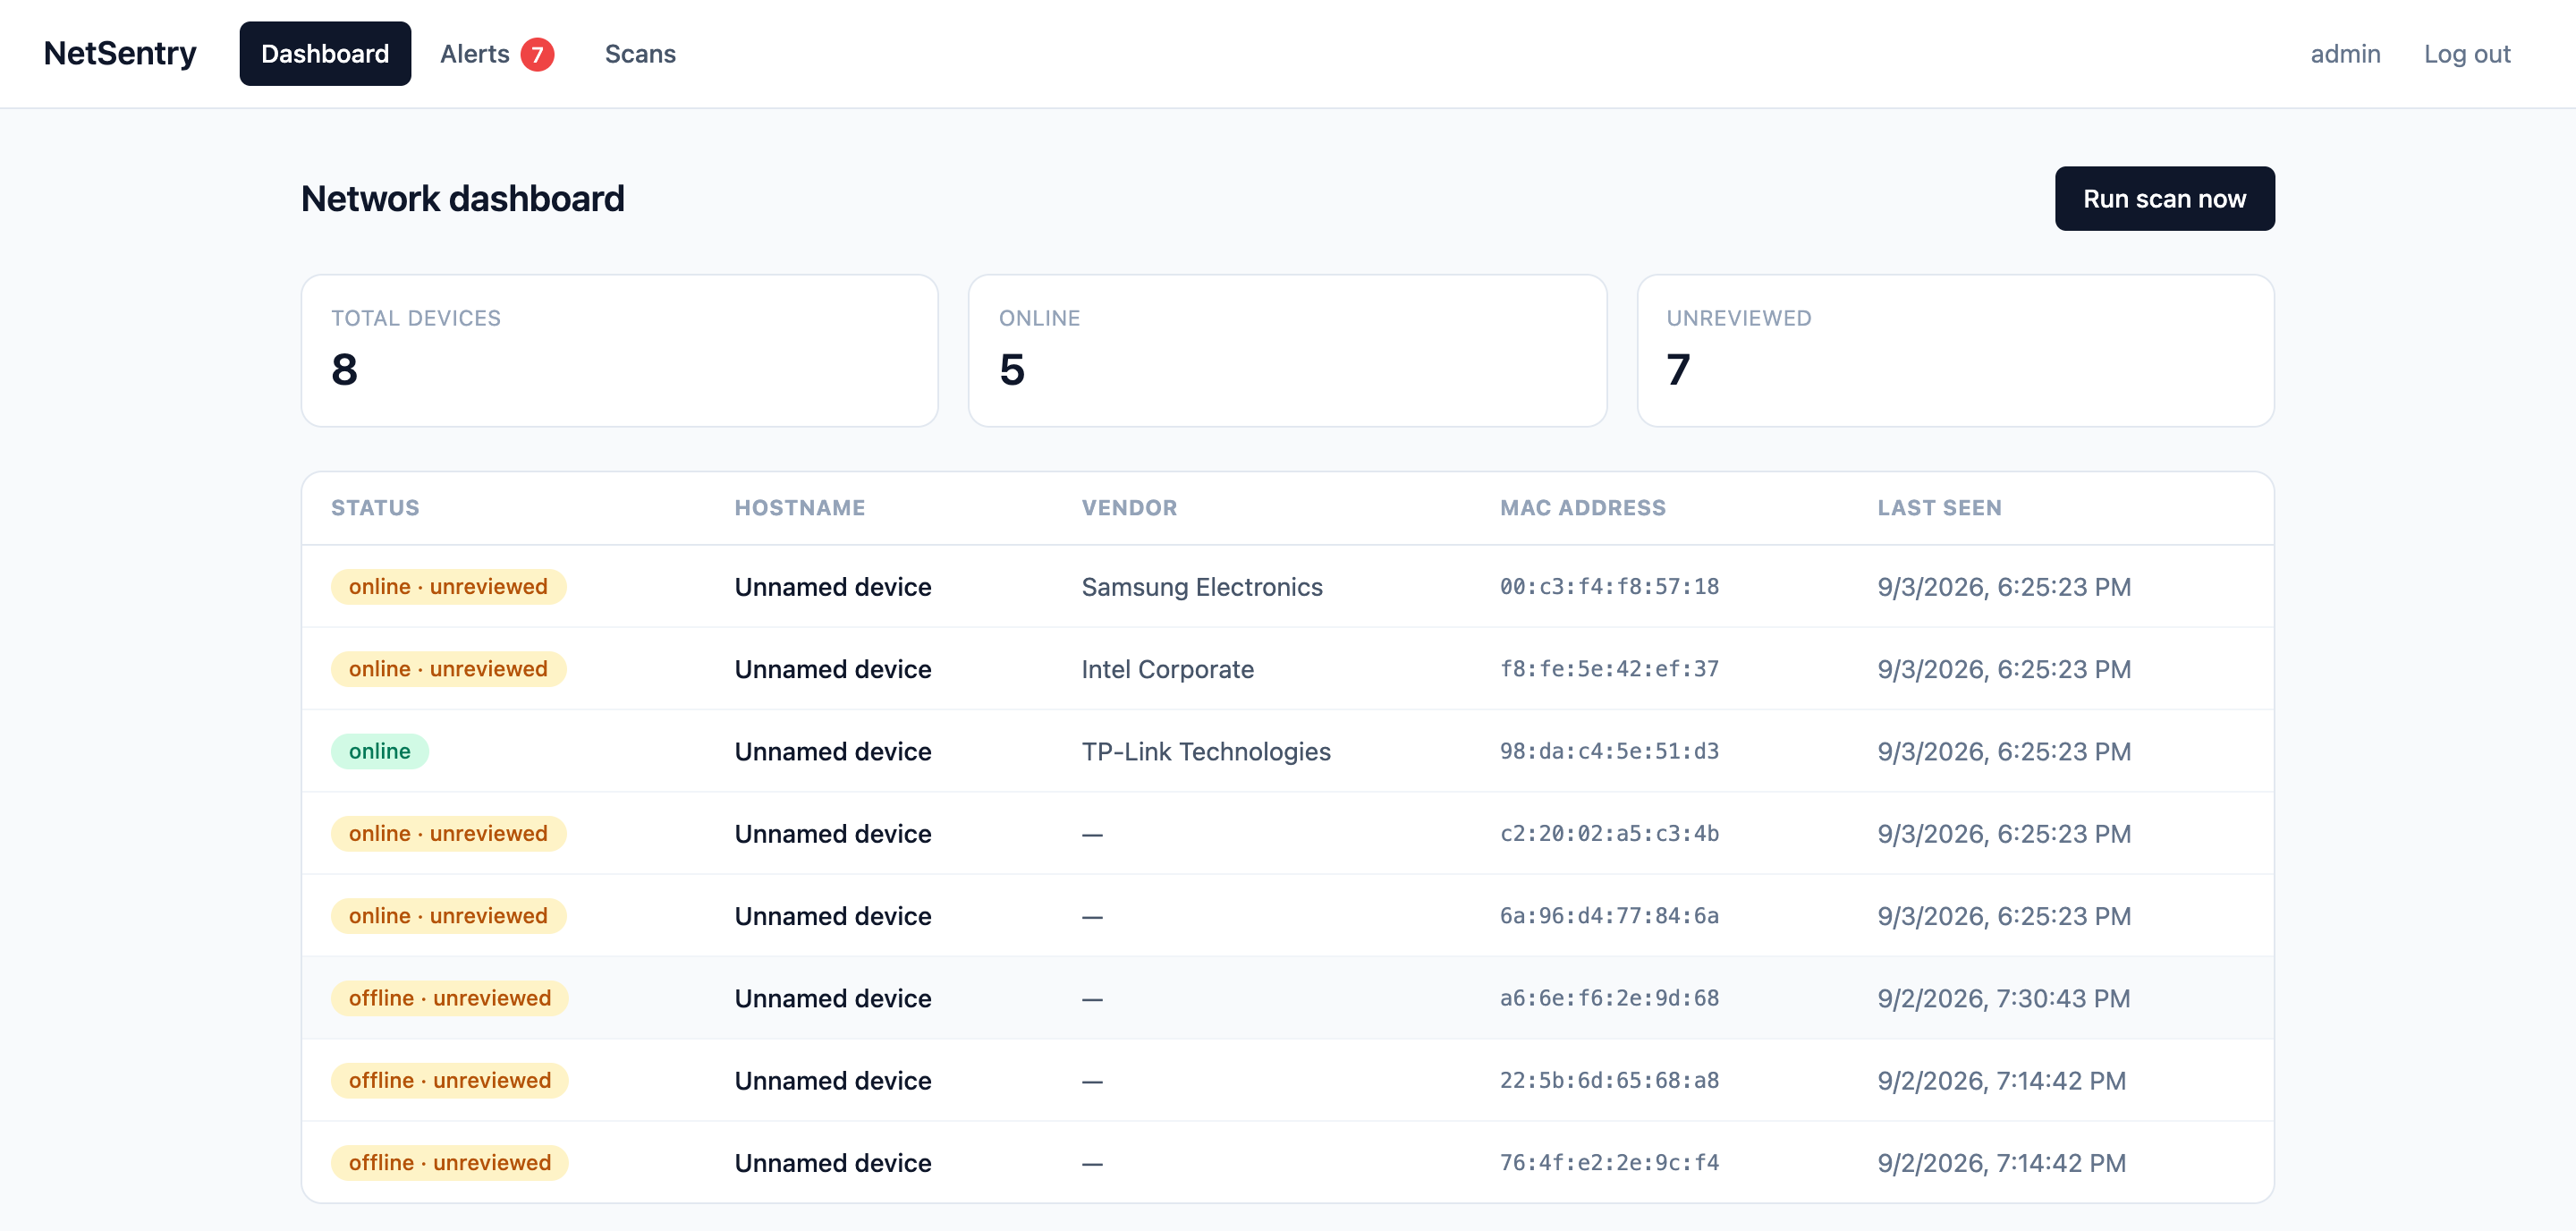
\includegraphics[width=\textwidth]{figuresChapitres/dashboard.png}
    \caption{Tableau de bord : vue d'ensemble des appareils détectés sur le réseau}
    \label{fig:dashboard}
\end{figure}

\section{Détail d'un appareil}

Le détail d'un appareil retrace son historique de détection au fil des scans successifs
(adresse IP observée, ports ouverts, date de détection), et permet à l'administrateur IT
de le marquer comme connu (liste blanche), ce qui met fin aux alertes futures pour cet
équipement.

\begin{figure}[htbp]
    \centering
    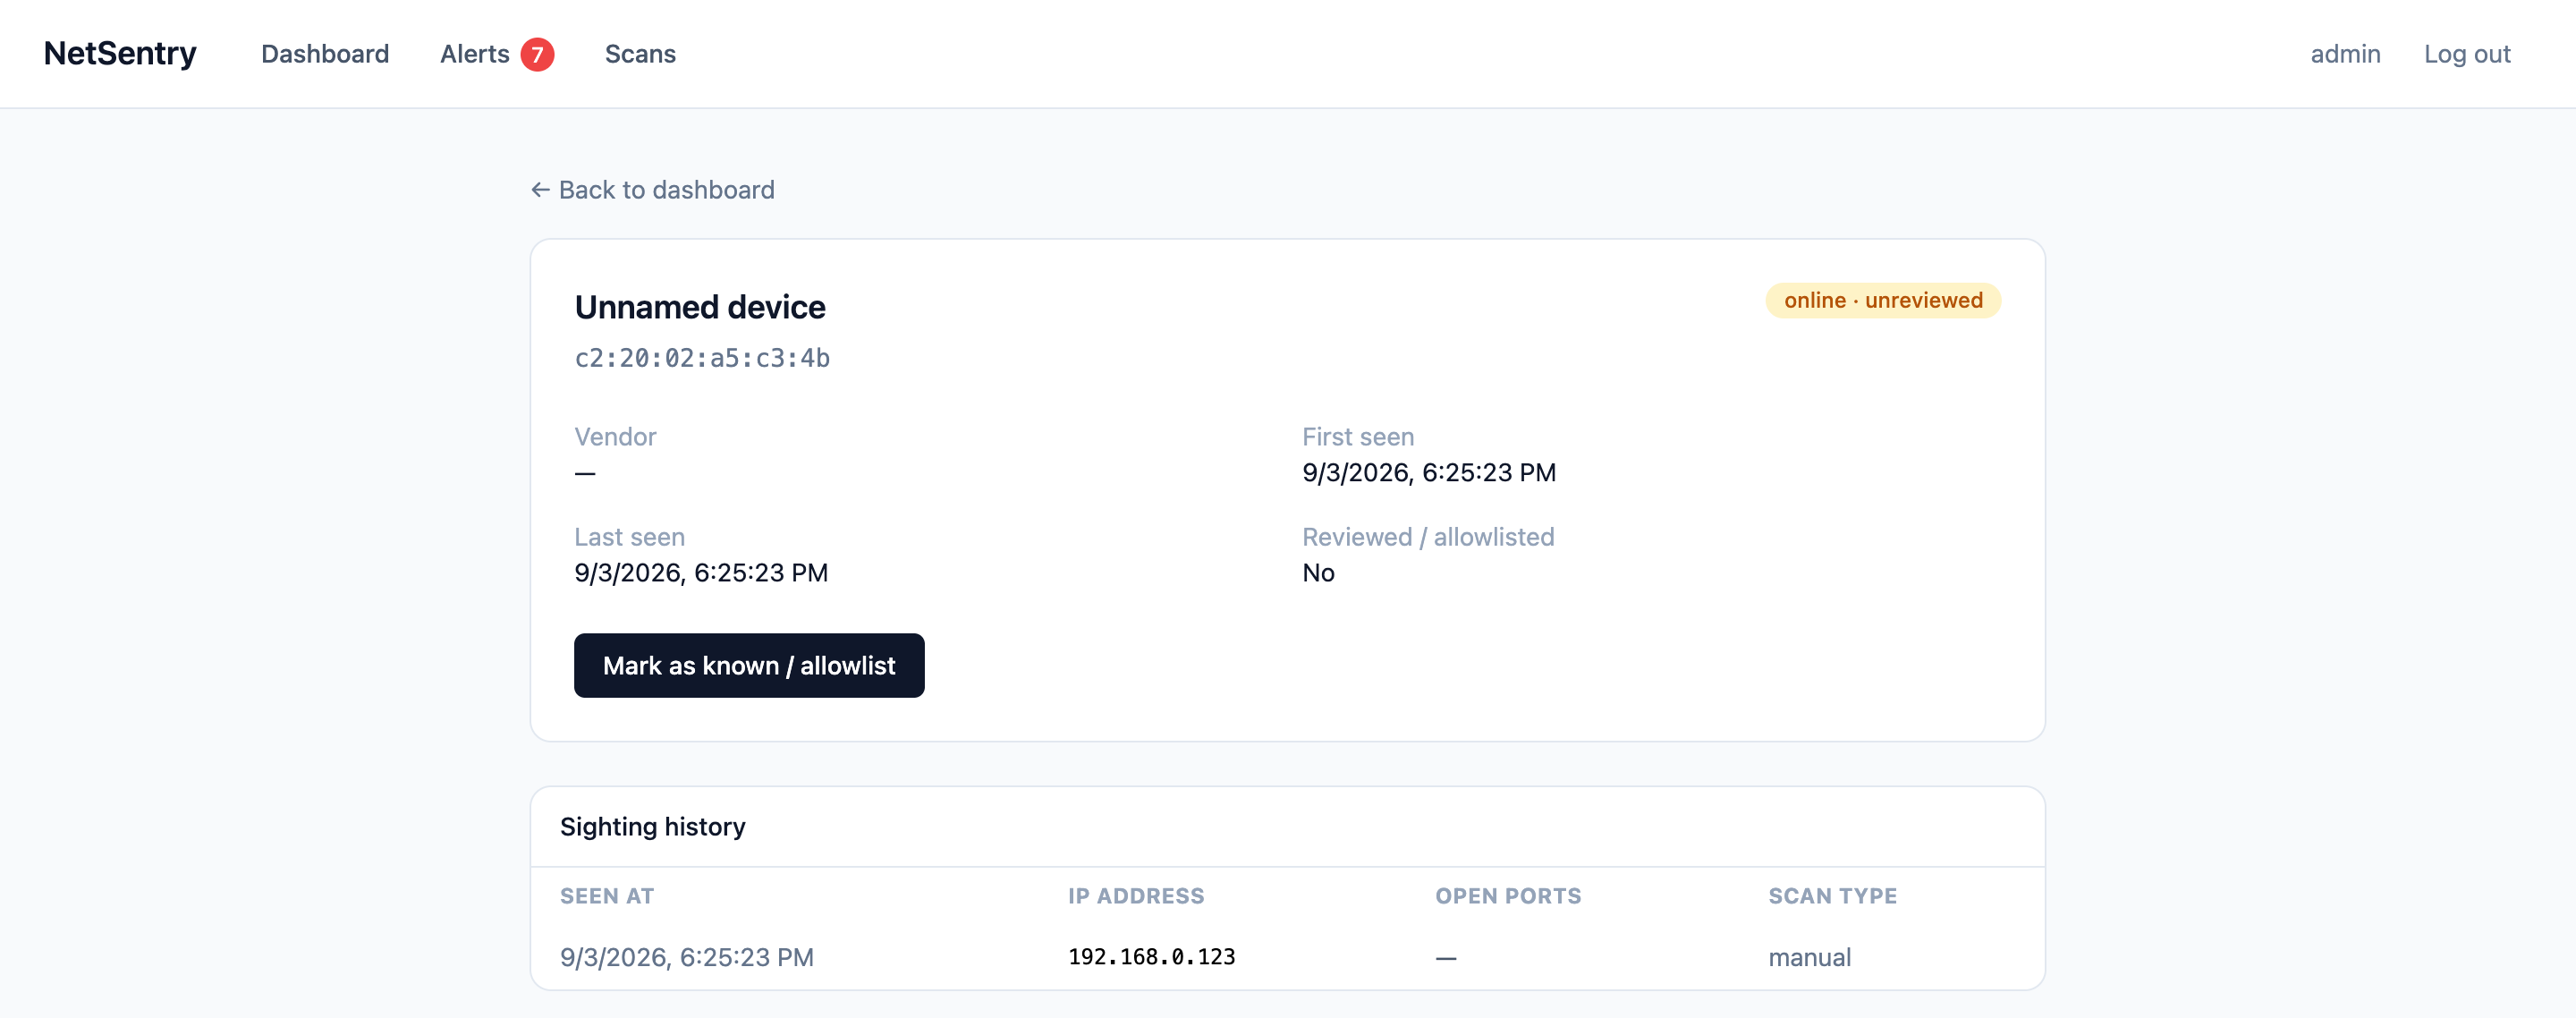
\includegraphics[width=\textwidth]{figuresChapitres/device_detail.png}
    \caption{Détail d'un appareil : historique de détection et mise en liste blanche}
    \label{fig:device-detail}
\end{figure}

\section{Alertes}

La page des alertes liste les appareils non reconnus signalés après un scan.
Conformément à la politique retenue, une alerte est générée une seule fois, lors de la
première détection d'un appareil inconnu ; l'administrateur IT peut ensuite l'acquitter
ou classer l'appareil comme connu pour désactiver les alertes futures le concernant.

\begin{figure}[htbp]
    \centering
    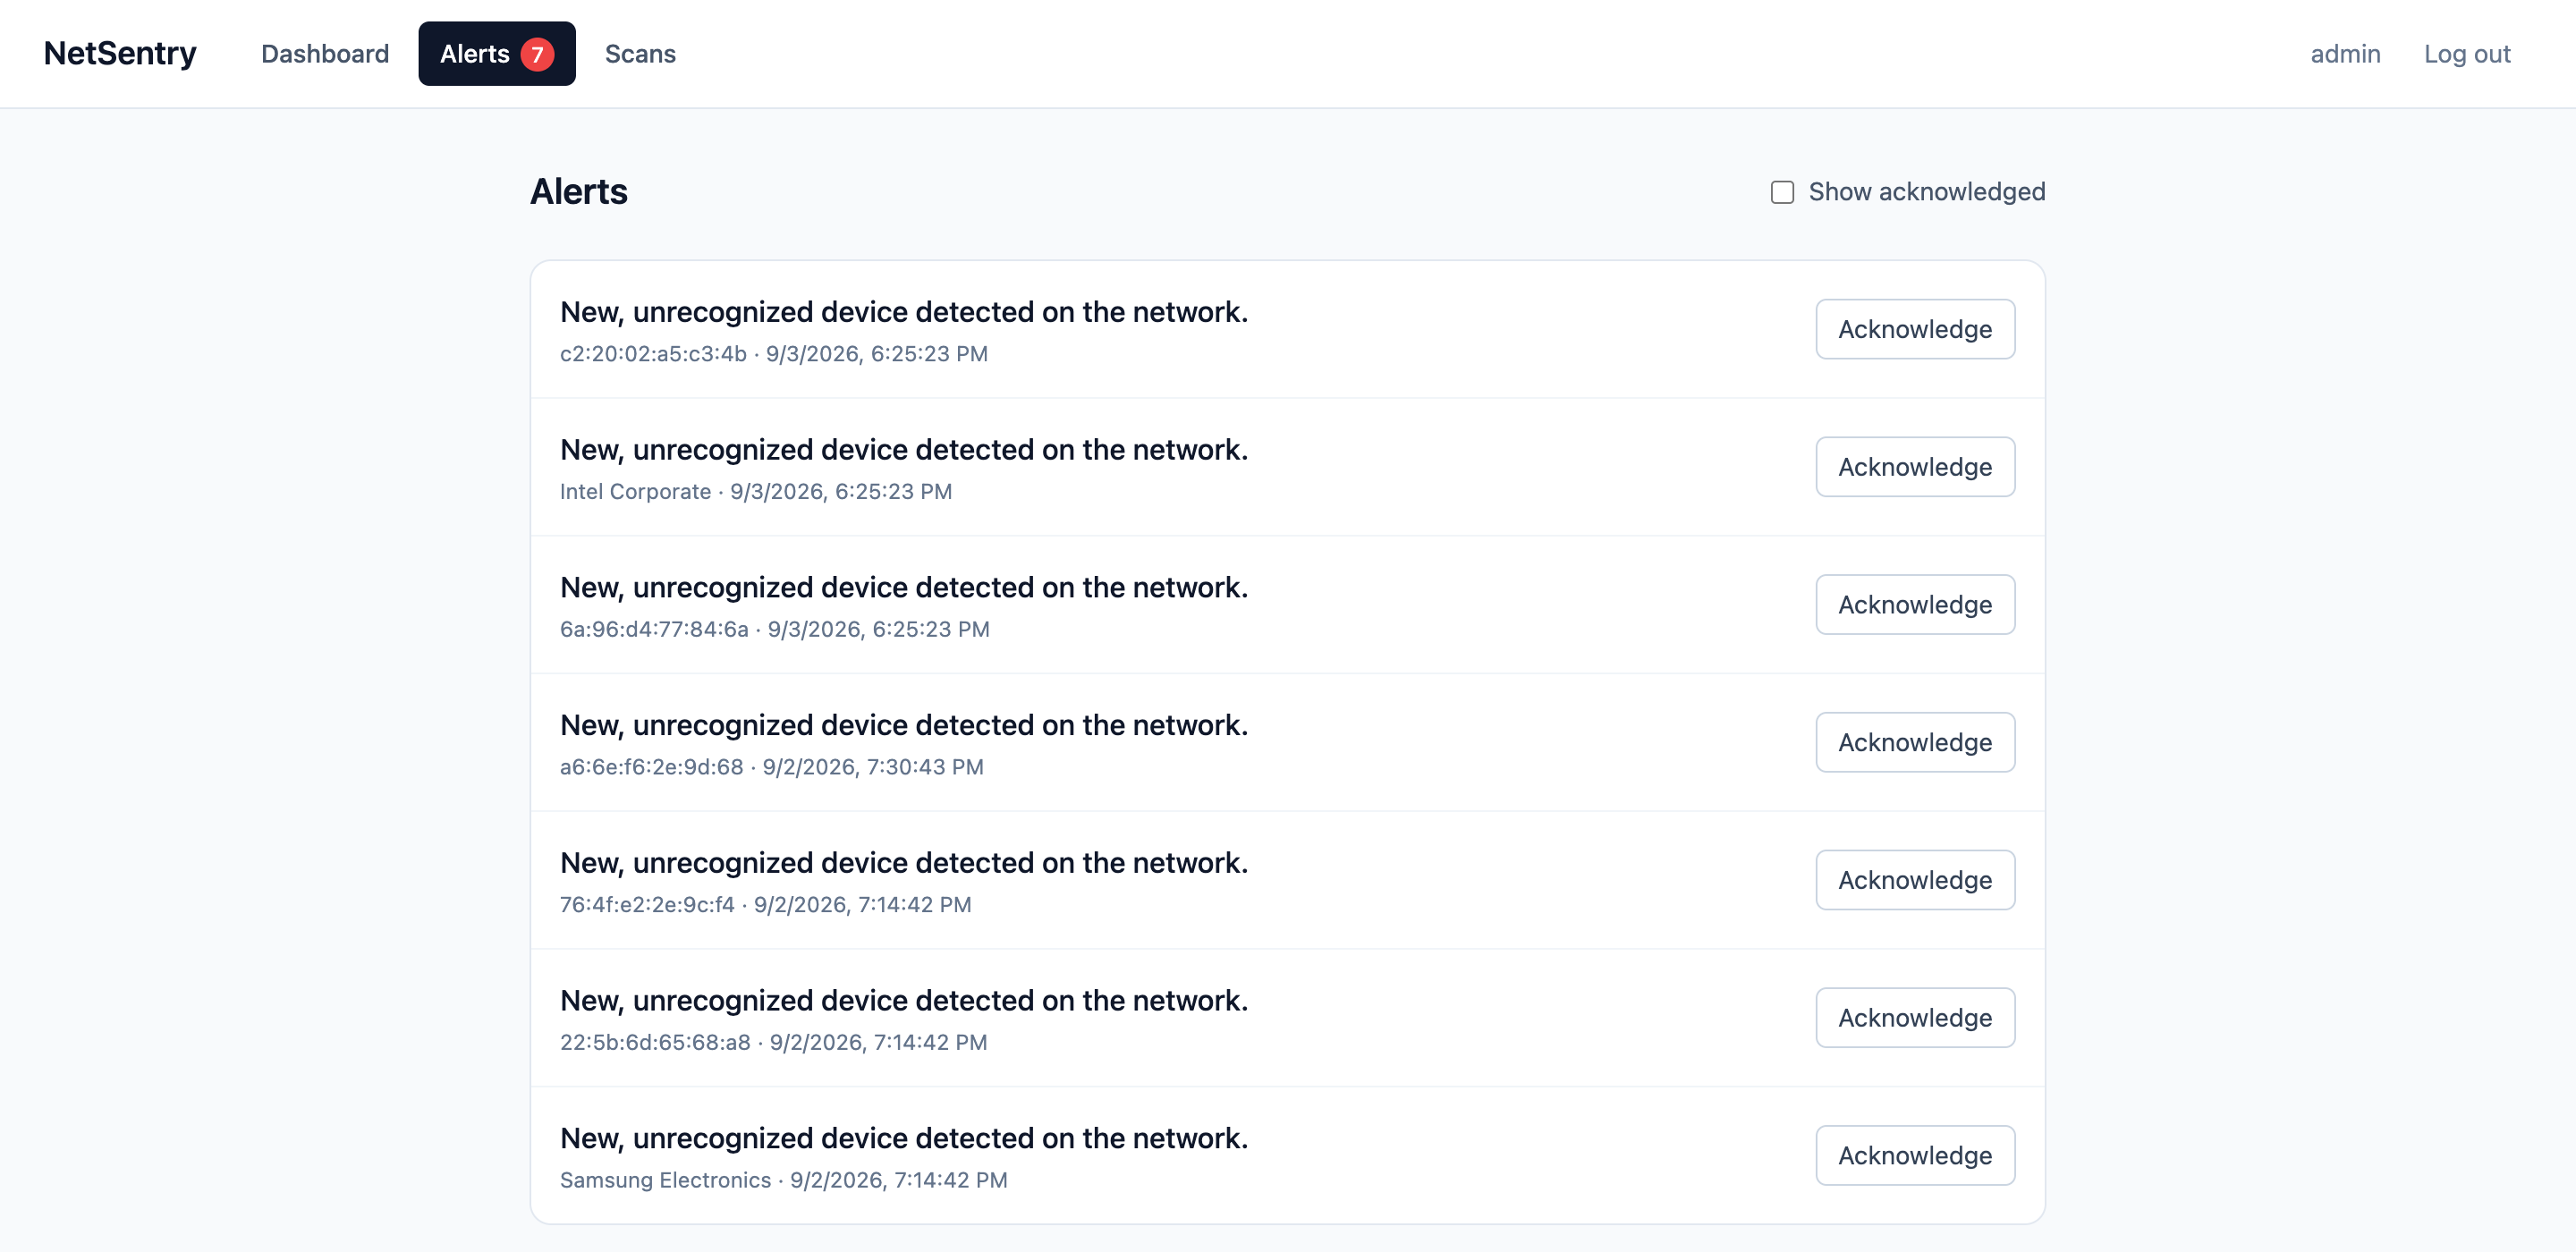
\includegraphics[width=\textwidth]{figuresChapitres/alerts.png}
    \caption{Alertes : appareils non reconnus signalés après un scan}
    \label{fig:alerts}
\end{figure}

\section{Historique des scans}

L'historique des scans conserve la trace de chaque exécution, manuelle ou planifiée,
avec son statut, le nombre d'hôtes trouvés et, le cas échéant, le message d'erreur
associé.

\begin{figure}[htbp]
    \centering
    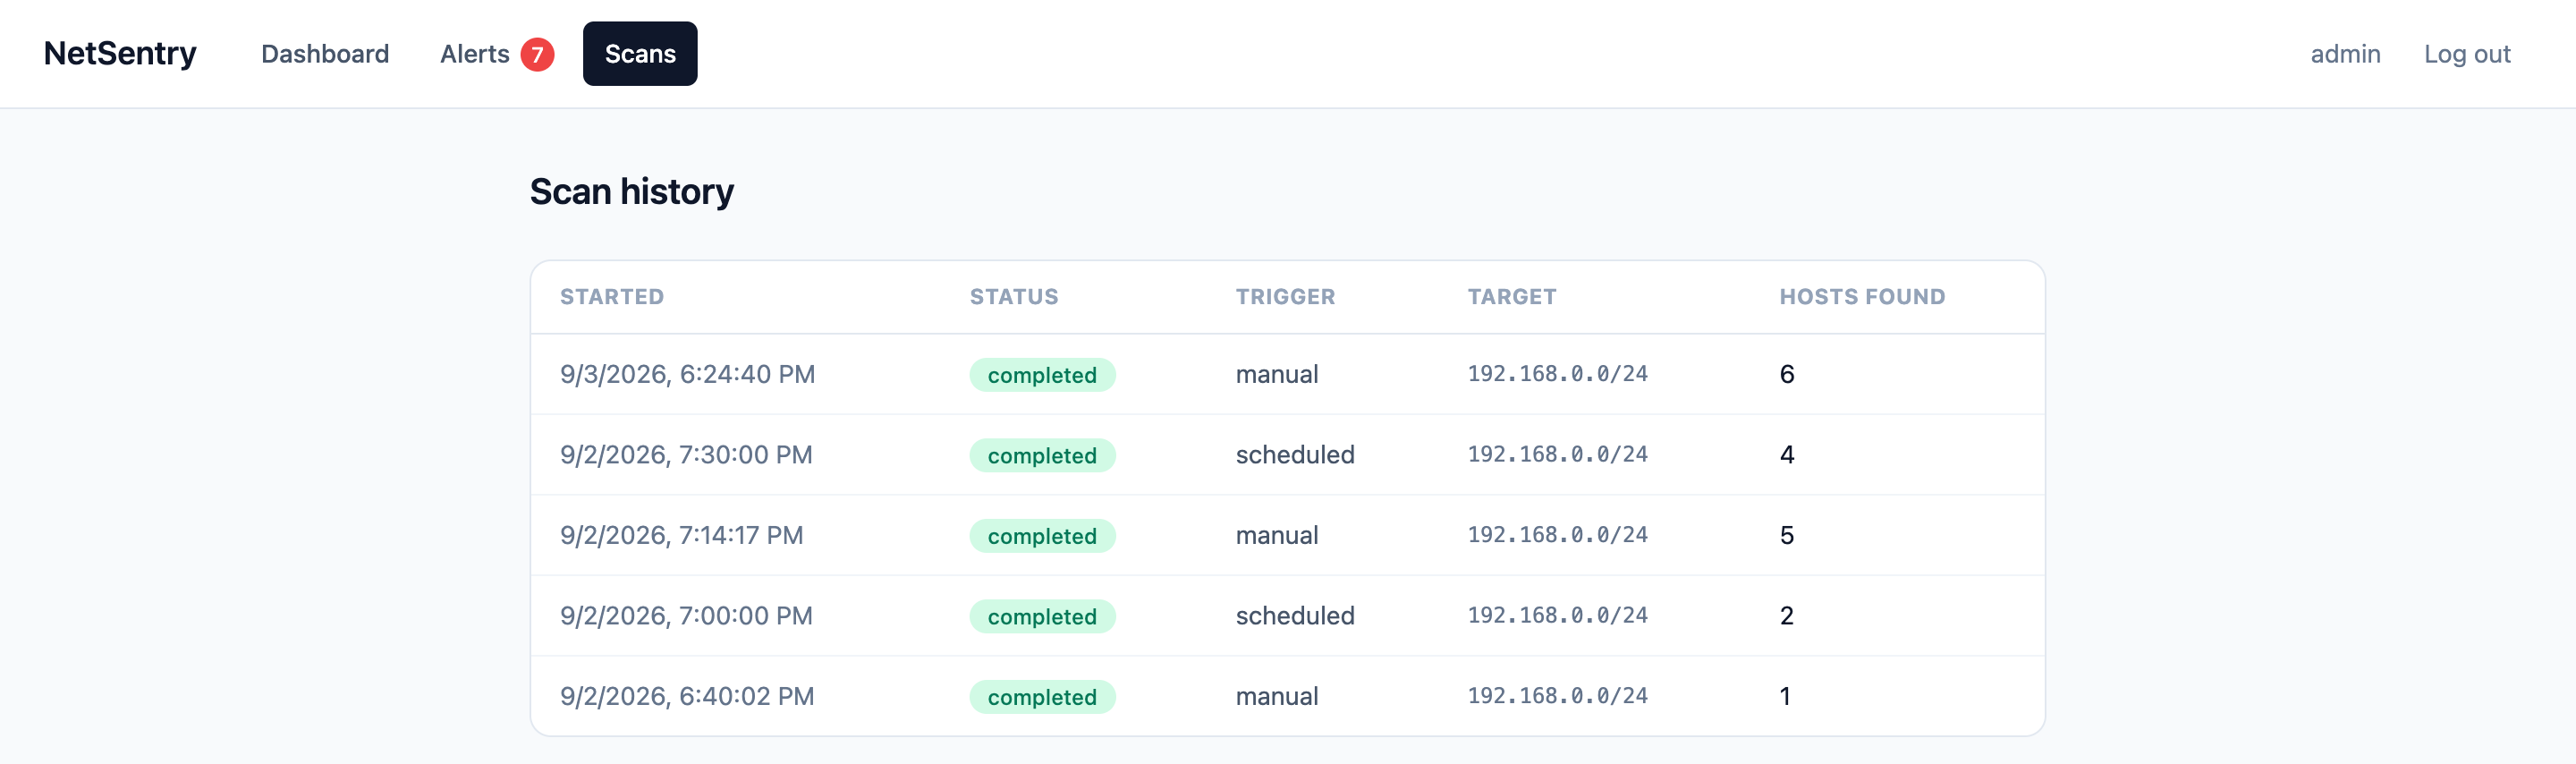
\includegraphics[width=\textwidth]{figuresChapitres/scan_history.png}
    \caption{Historique des scans exécutés (manuels et planifiés)}
    \label{fig:scan-history}
\end{figure}

\section{Versionnage}

Le projet est versionné avec Git et hébergé sur un dépôt GitHub public. L'historique
reste volontairement synthétique à ce stade du stage : un commit initial, l'ajout des
documents de cadrage, puis un commit unique regroupant la construction du MVP (backend,
frontend, conteneurisation). Il sera affiné par des commits plus granulaires au fil des
prochaines itérations.

\begin{figure}[htbp]
    \centering
    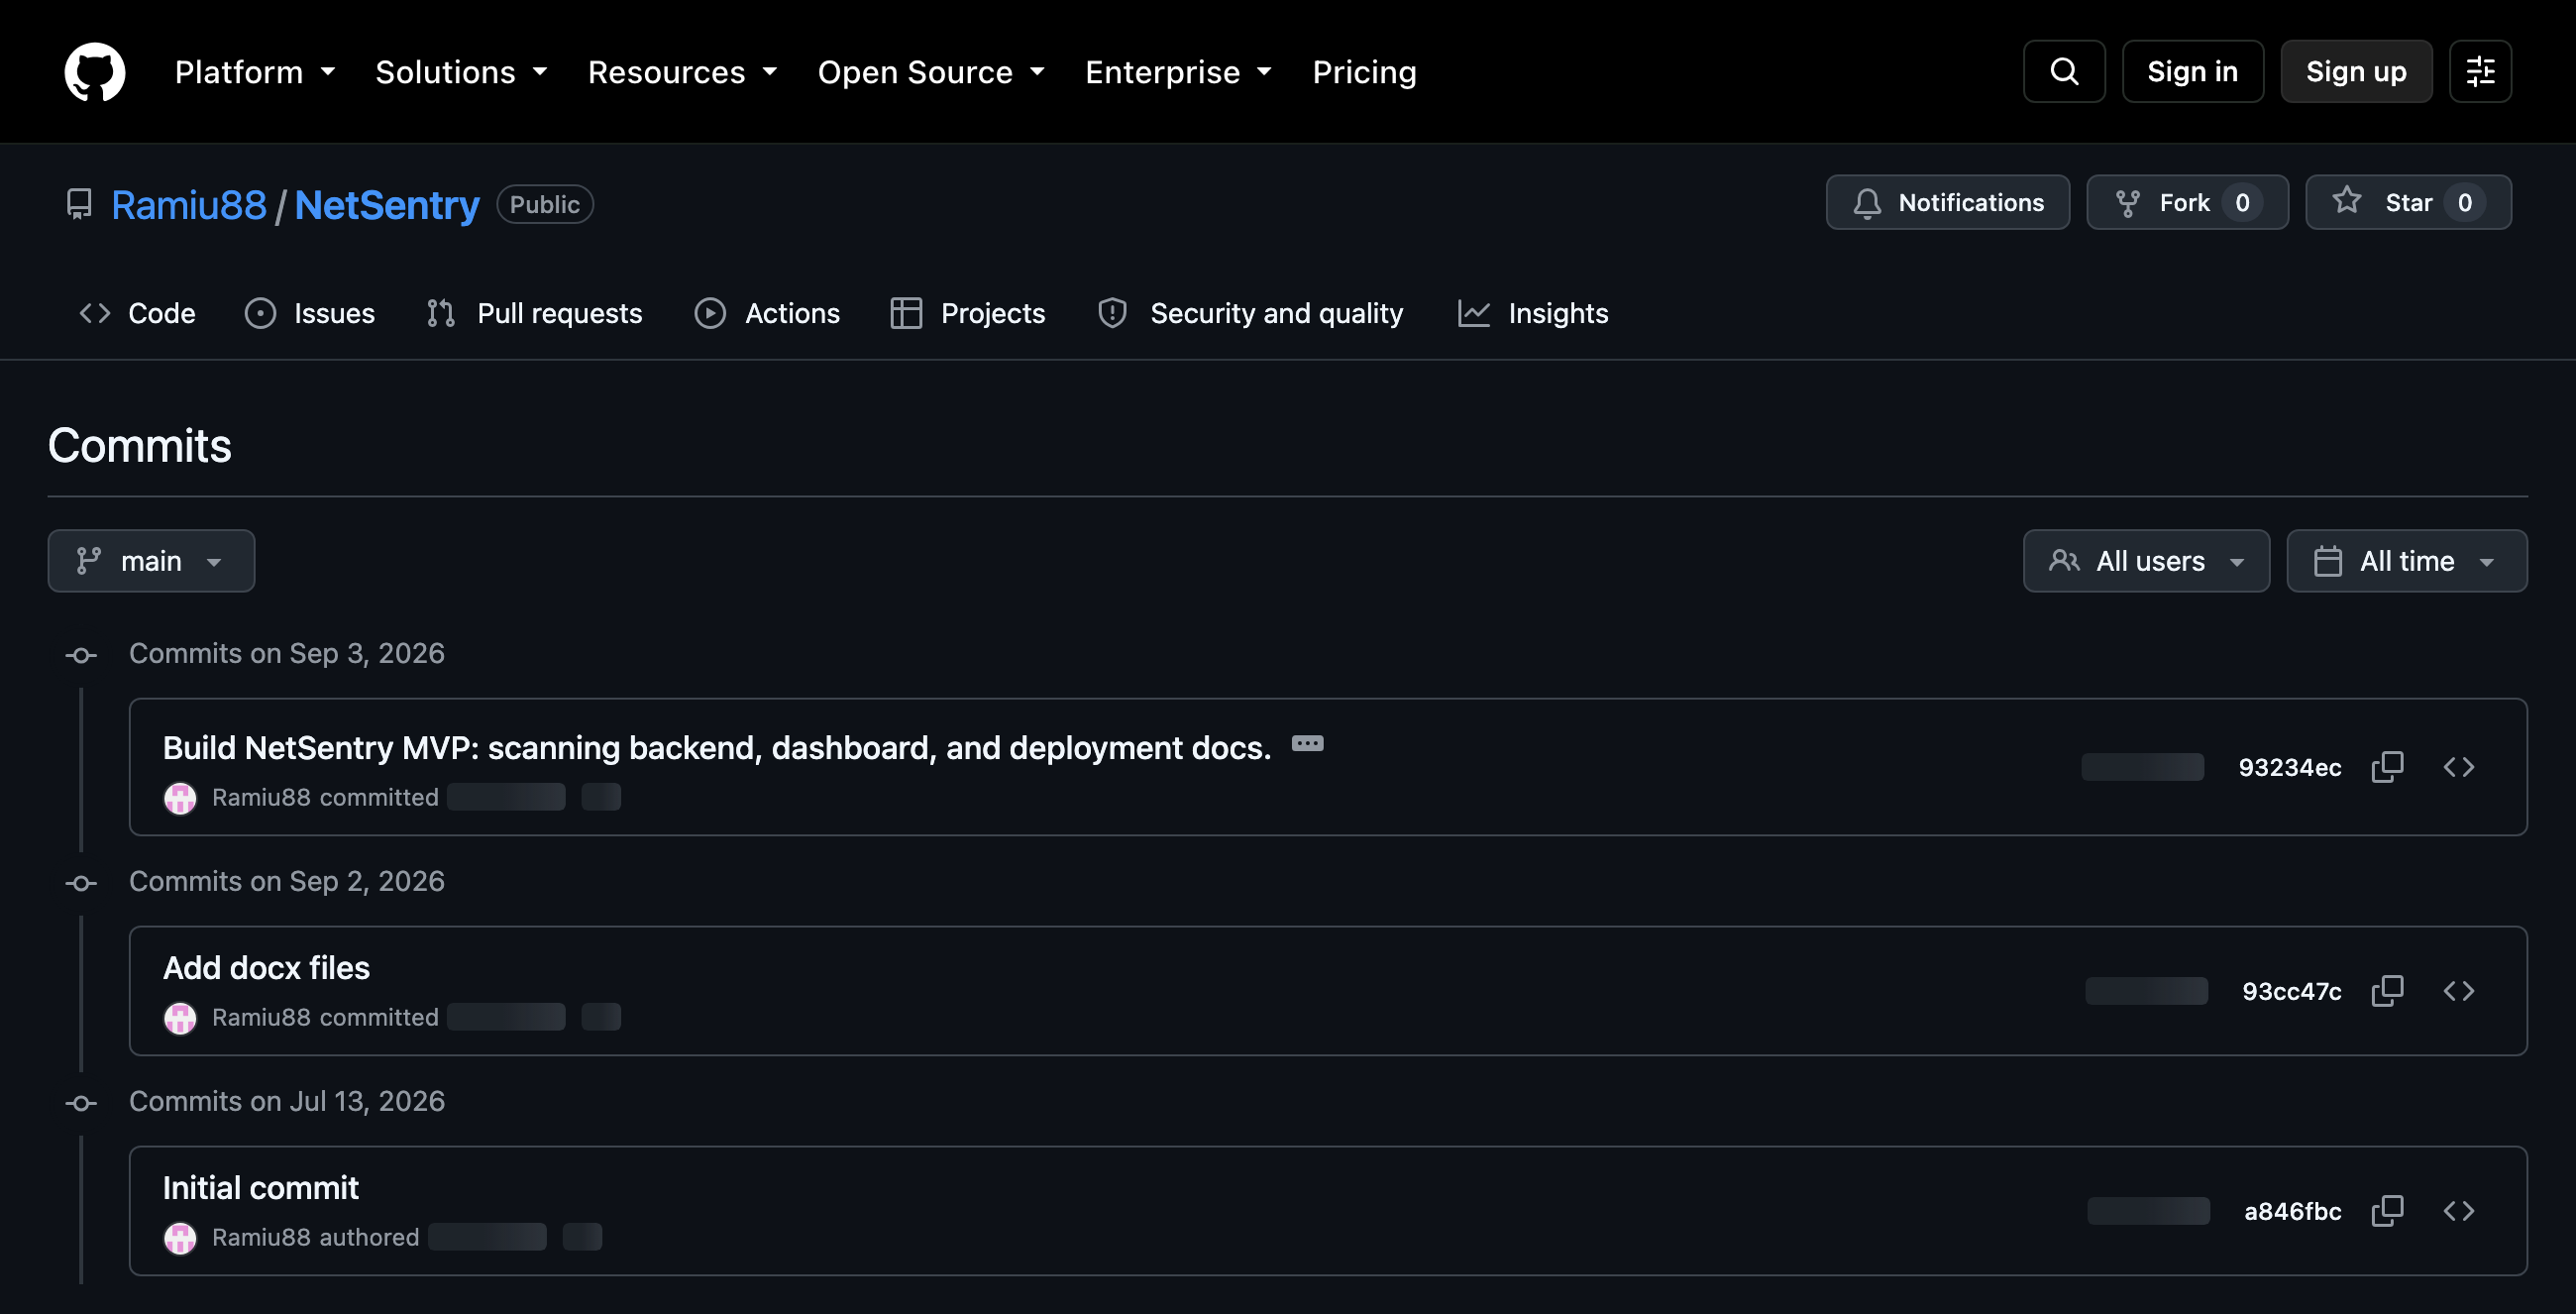
\includegraphics[width=\textwidth]{figuresChapitres/github_commits.png}
    \caption{Historique des commits du dépôt GitHub NetSentry}
    \label{fig:github-commits}
\end{figure}

\section{Conclusion}

Ces captures d'écran illustrent le fonctionnement réel et vérifié de la chaîne complète
de NetSentry, du scan réseau jusqu'à la restitution dans le tableau de bord. Elles
constituent la démonstration concrète des objectifs fixés au premier chapitre.
